\section{PDF: Structure, Complexity, Vulnerabilities}

\subsection{PDF Structure}

\begin{figure}[t]
    \centering
    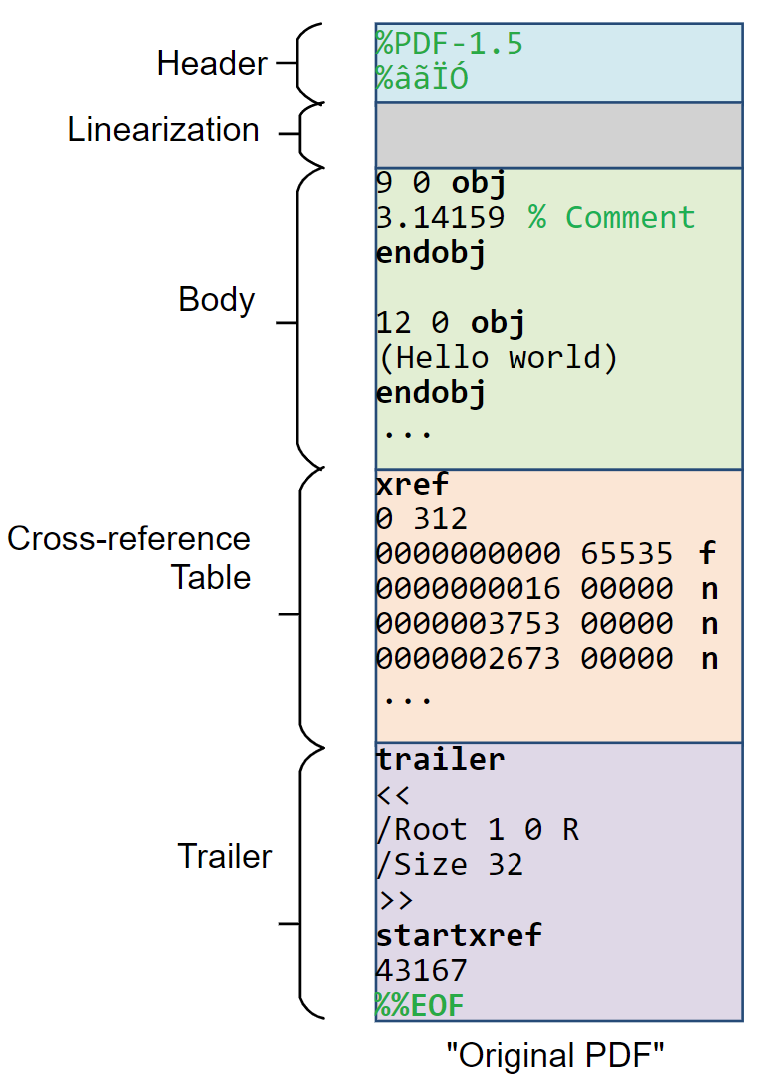
\includegraphics[width=0.35\linewidth]{figures/pdf-structure.png}
    \caption{PDF File Structure.}
    \label{fig:pdf-structure}
\end{figure}

The overall structure of a PDF is shown in \cref{fig:pdf-structure}.
\todo{short paragraph: describe overall PDF doc structure}

\todo{PW: more detail}
  
\todo{import the type definitions?}

\subsection{Root Causes of PDF Complexity}

Most data formats can be described by much simpler mechanisms;
most language processors (e.g., a Python parser) can be described and parsed by
textbook methods (e.g., the old \emph{lex} and \emph{yacc} are sufficient for
most language processors);
so what makes PDF processing so much more complex?
\begin{lstlisting}[style=meta]
  - indirect offsets
    - which may recursively point to other indirect offsets
    - need programming language
      (or a 'seek' in the data definition lang)
  - DOM is a directed graph structure that allows cycles and arbitrary references (so not a DAG)
    - objects point to objects via byte offsets (cf. not by nested expressions such as XML)  
  - backwards parsing
  - some parsing rules written as to be not relevant to parsers ("writer-only rules")
  - incremental updates as a set of deltas to be applied to the file, which change the DOM
    - (note: unlike HTML, PDF's DOM is fixed and cannot be altered by JS)
  - xref tables ...
  - ... giving rise to cavities
    - giving rise to polyglots
  - dependent parsers
  - <MORE?>
\end{lstlisting}

Further detail of how these work in PDF is in \cref{sec:specifying}.

% ------------------------------------------------------------------------------
\subsection{Pre-DOM Vulnerabilities \note{1pp}}
\label{sec:predom-vulnerabilities}

As will become even more apparent, there is a significant amount of
parsing and computation that needs to be done \emph{pre-DOM}.
And given our recent points about the \emph{PDF Trust Chain}
(\cref{sec:trust-chain}),
it should not surprise us that most of the PDF attack vectors
(\cref{sec:pdf-vulnerabilities})
involve some aspect of breaking the \emph{DOM} abstraction.
I.e., they occur at the \emph{pre-DOM} levels.

{\bf{Shadow Attacks}} \todo{...}

{\bf{Schizophrenia}} \todo{should define what we mean by schizo - is this the same thing that gives rise to parser differentials or a feature of of the syntax or layout of PDF?}
\begin{lstlisting}[style=meta]
  - writer errors
  - parser differentials
    - e.g., ignoring xref tables
  - recovering parsers !!
  - blind faith in incremental updates (Shadow Attacks)
\end{lstlisting}

{\bf{Polyglots}} 
\todo{... arising from cavities and permissive implementations and ...}
\begin{lstlisting}[style=meta]
- Multiple places for hidden/unused/malicious data in PDF
  - non-obvious places, unnoticed when "simply parsing"
  - e.g., shadow-attacks
  - dead bytes, dead objects, dead updates, dead linearization sections, etc.
\end{lstlisting}

{\bf{Denial of Service (DOS)}} 
%
\begin{lstlisting}[style=meta]
- [potential recursion many places]
- format may not be well-defined because the recursion is not
    "well-defined"
\end{lstlisting}


{\bf{Others}} \todo{Maybe PII/redaction issues - just 'cos you delete something in a PDF doesn't mean it is really deleted (thanks to incremental updates)!!!! }
